\documentclass[10pt,journal,compsoc,fleqn]{IEEEtran}
\usepackage{graphicx}
\usepackage{amsmath}
\usepackage{amsfonts}
\usepackage{epstopdf}
\usepackage{url}
\usepackage{CJKutf8}
\usepackage{algorithm, algorithmic}
\newtheorem{thm}{{Theorem}}[section]
\newtheorem{defn}{Definition}[section]
\newtheorem{lem}{Lemma}[section]
\newtheorem{rmk}{Remark}[section]
\newenvironment{proof}{\noindent {\bf Proof: }}\\


\hyphenation{op-tical net-works semi-conduc-tor}


\begin{document}
\begin{CJK}{UTF8}{song}
\title{Work}
\author{龙威帆}
\maketitle

地址:\url{https://github.com/az2181036/seclass}
\section*{运行结果}
1.初始图(Fig. \ref{init})
\begin{figure}[H]
  \centering
  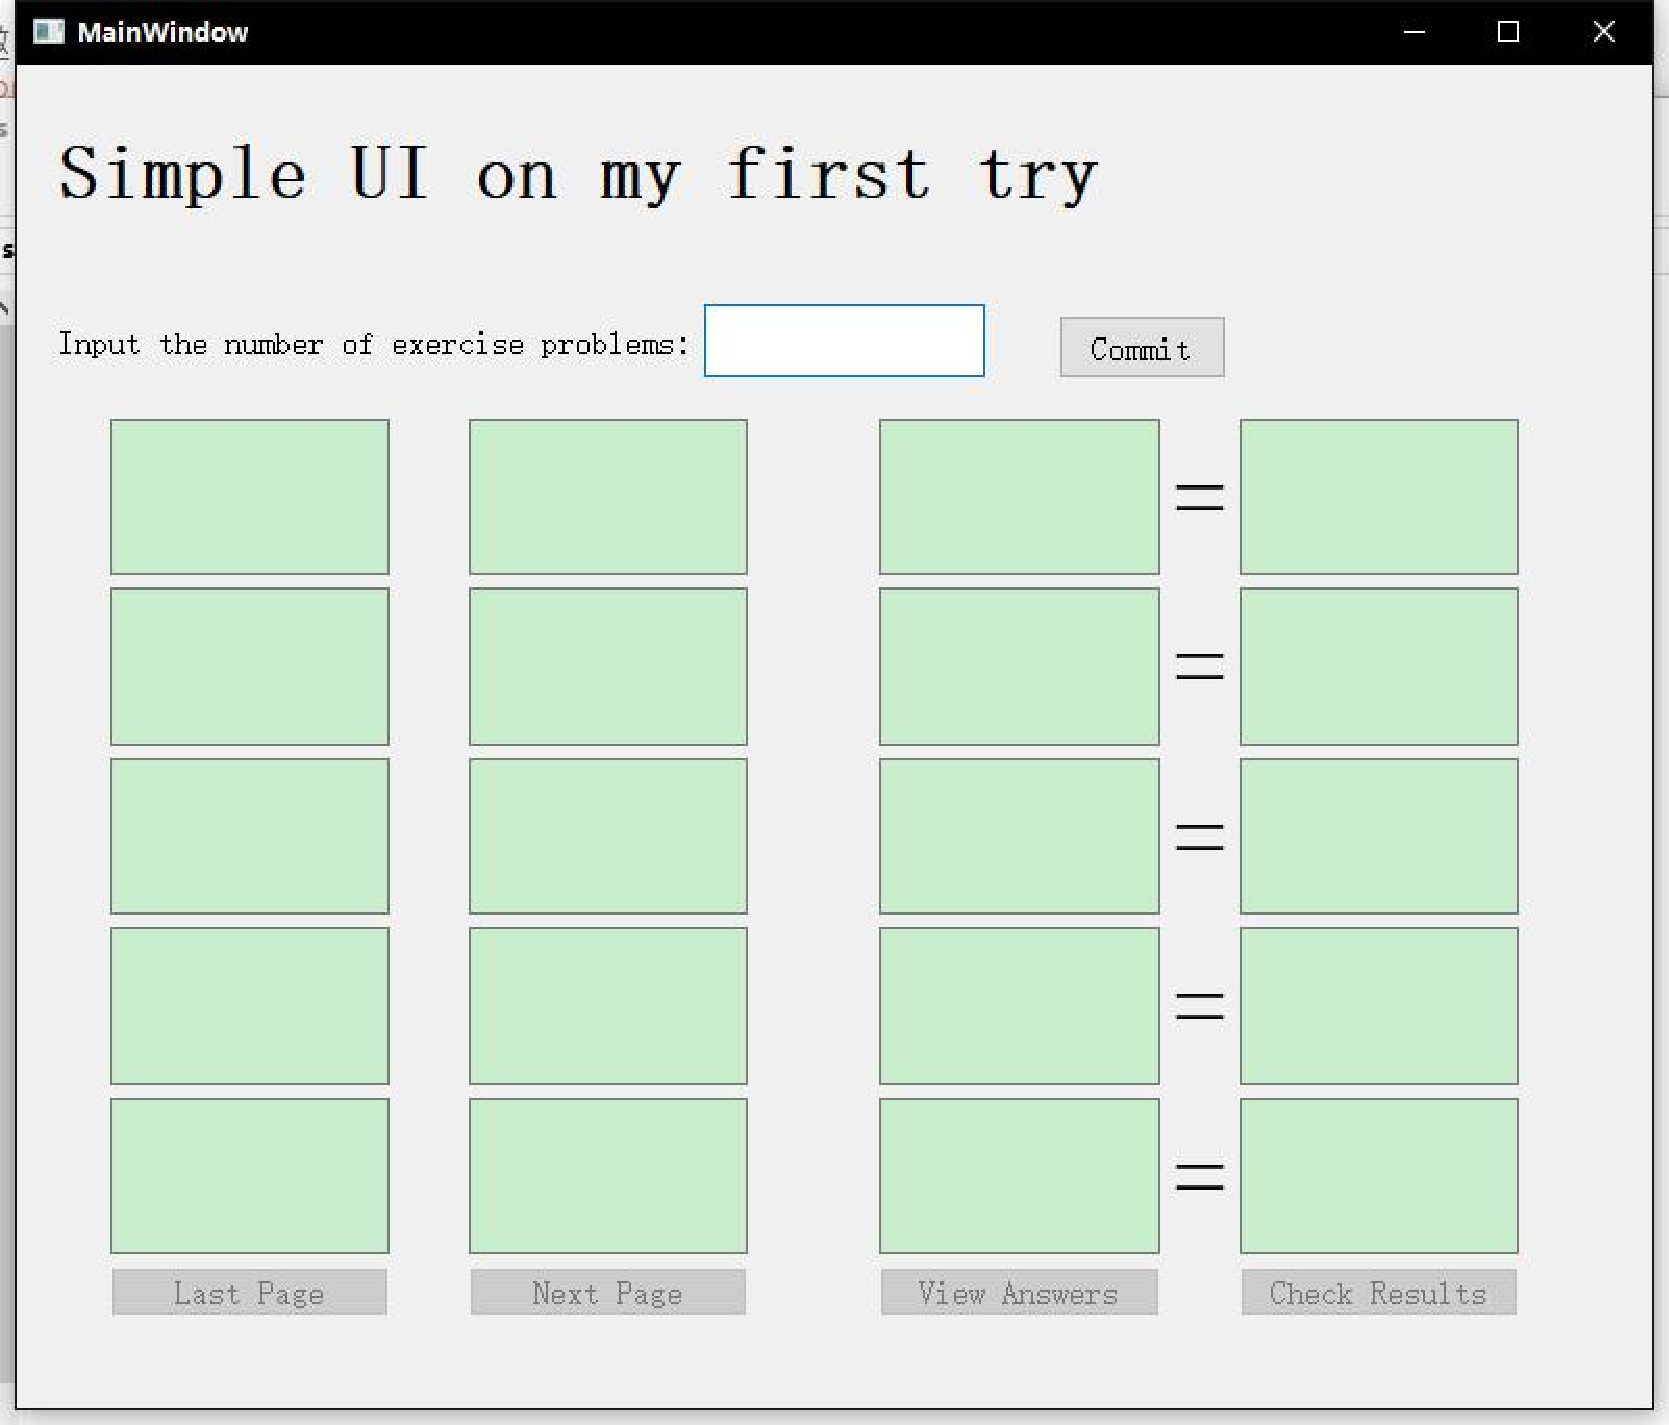
\includegraphics[width=2.5in]{./figures/init.pdf}
  \caption{Init}
  \label{init}
\end{figure}
\noindent 2.输入18, 提交(Fig. \ref{Commit}):
\begin{figure}[H]
  \centering
  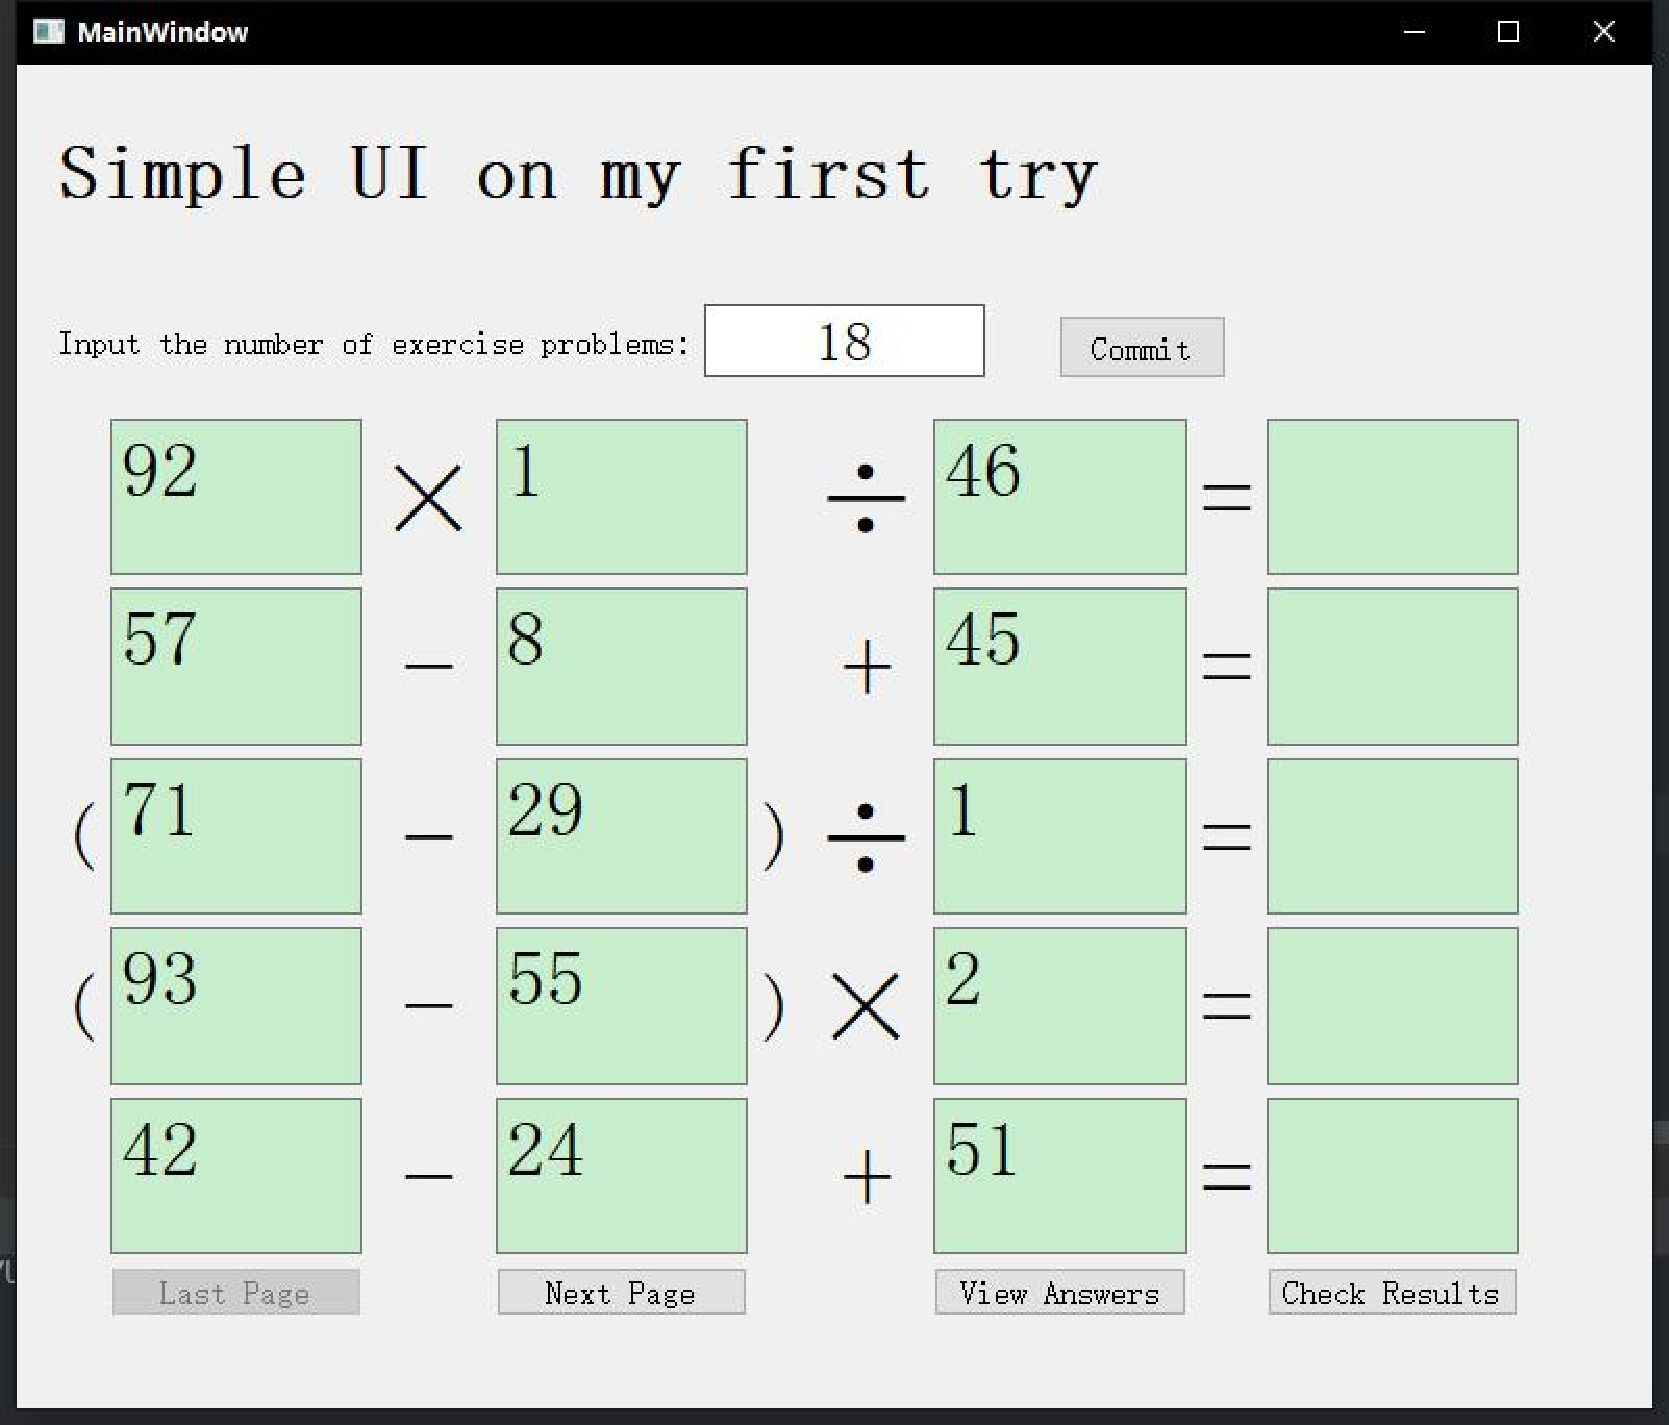
\includegraphics[width=2.5in]{./figures/commit.pdf}
  \caption{Commit}
  \label{Commit}
\end{figure}
\noindent 3.输入两个数在等号后的框中,点击 check results按钮(Fig. \ref{check_rst}):
\begin{figure}[H]
  \centering
  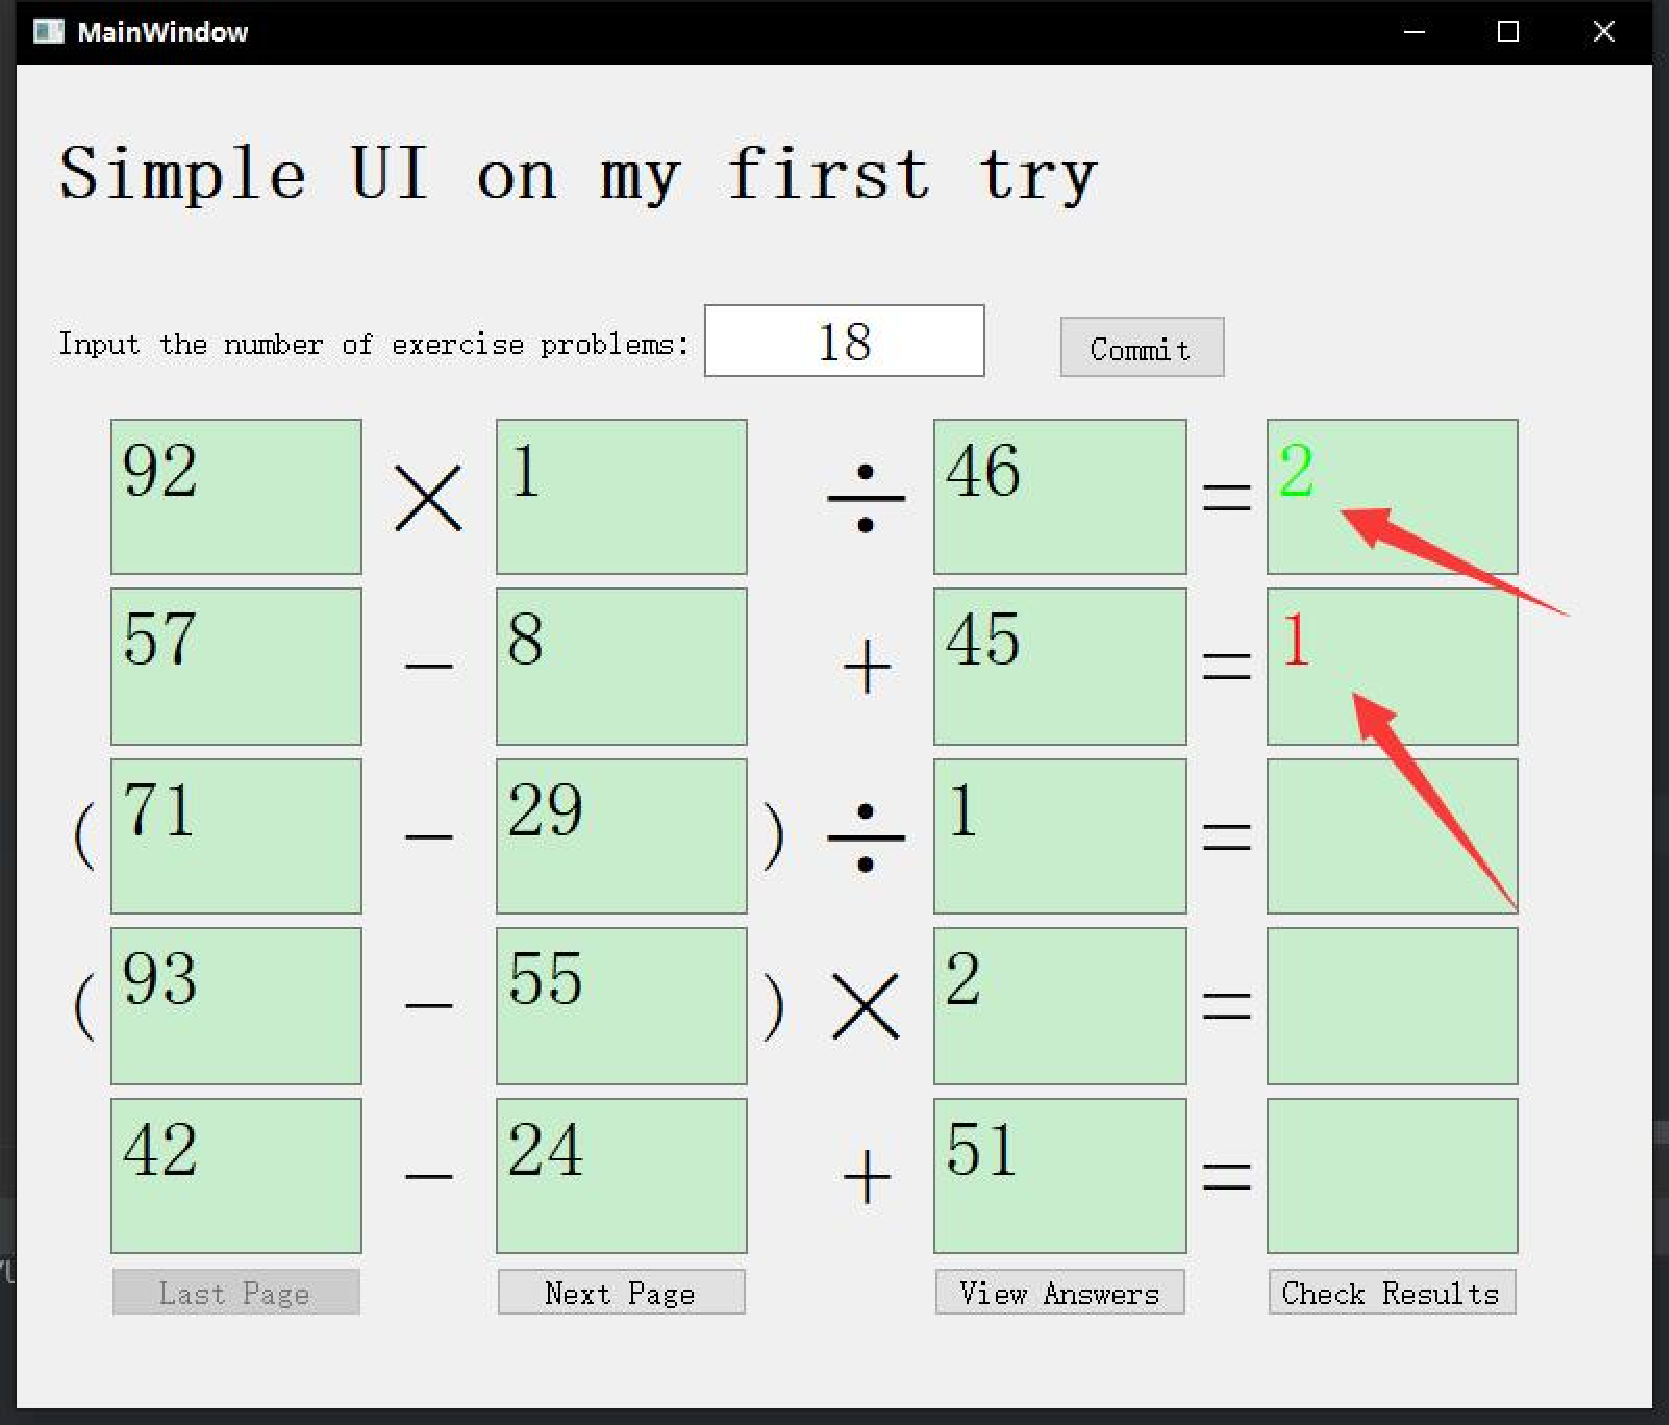
\includegraphics[width=2.5in]{./figures/check_rst.pdf}
  \caption{check results}
  \label{check_rst}
\end{figure}
\noindent 4.显示答案,点击 view answers按钮(Fig. \ref{view_asw}):
\begin{figure}[H]
  \centering
  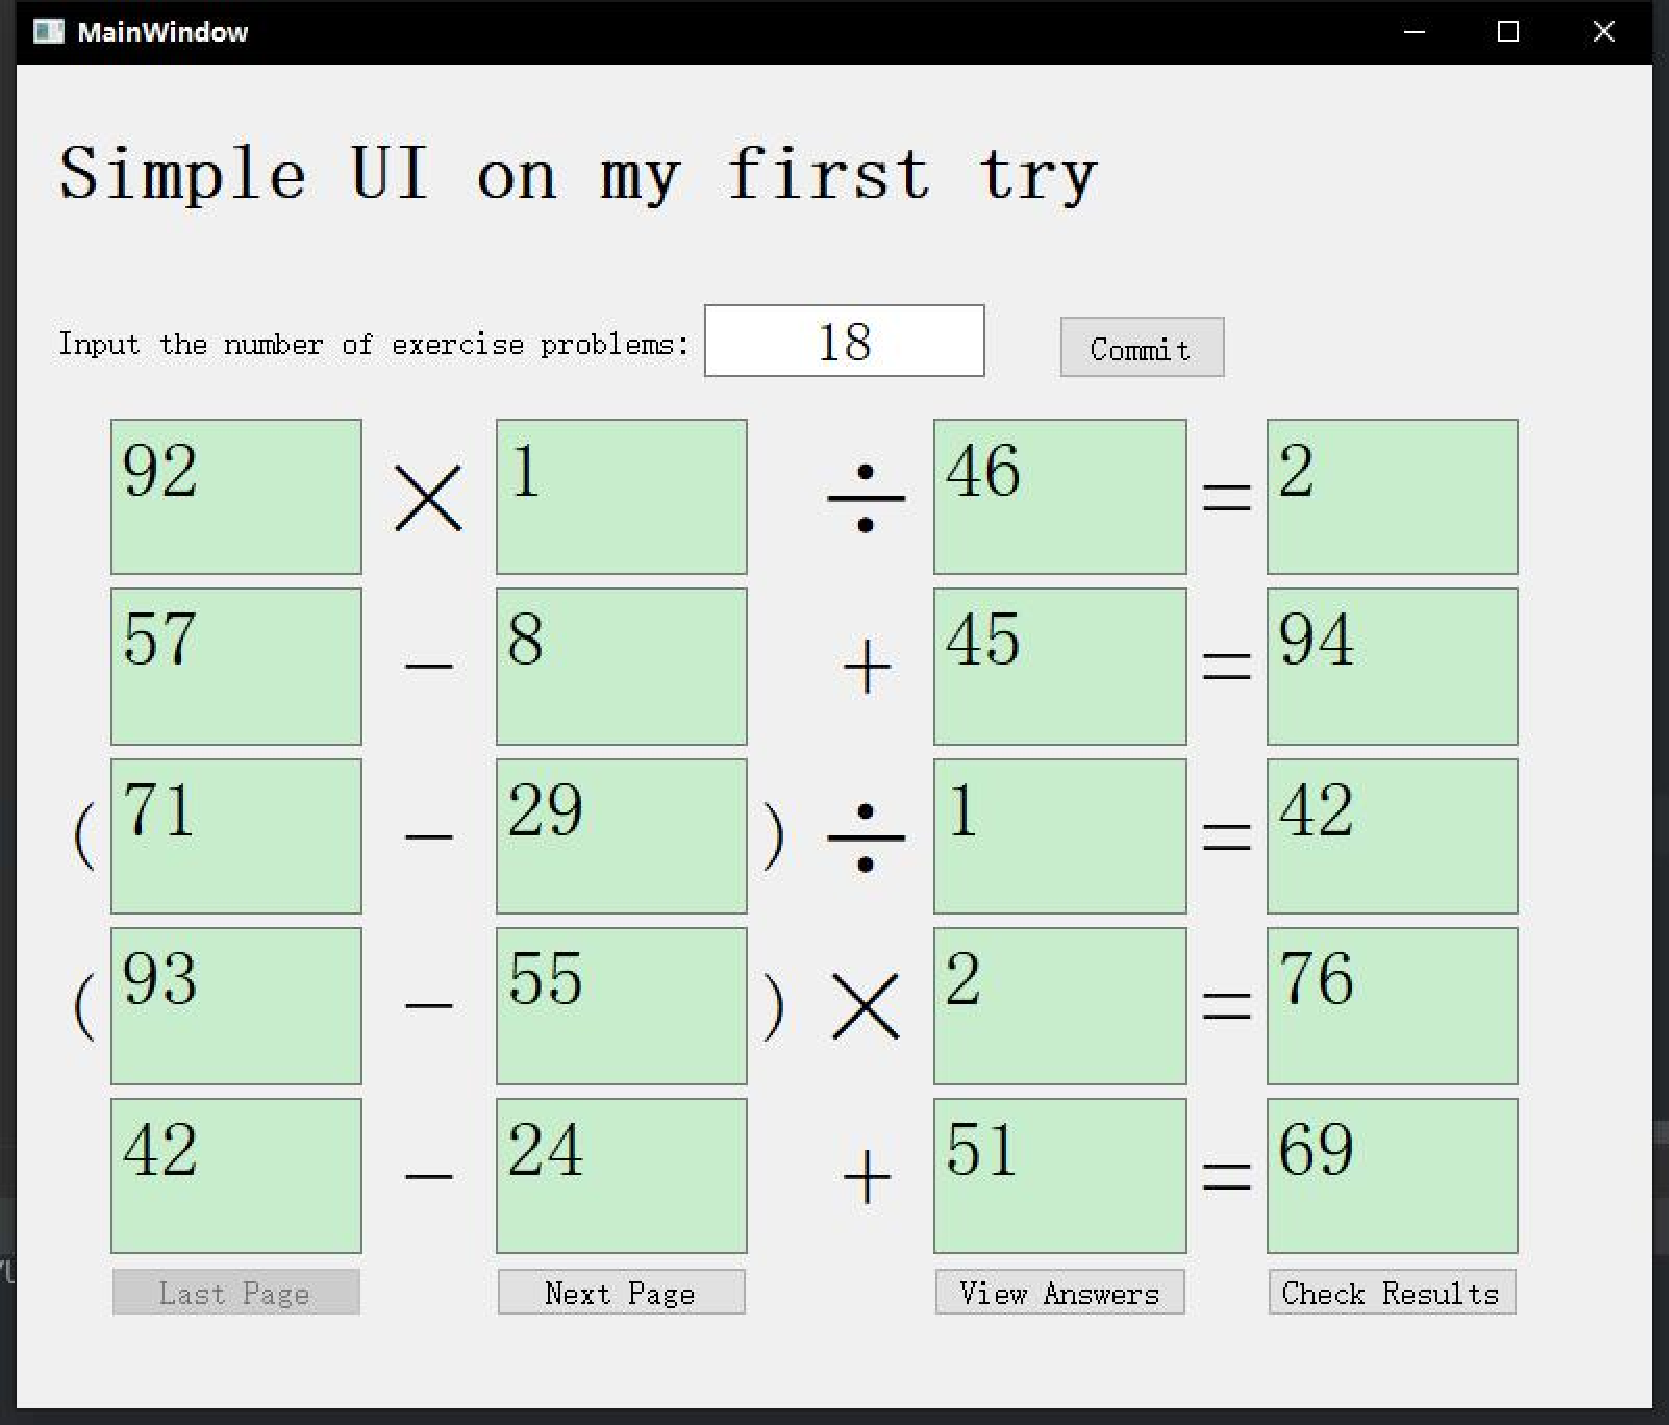
\includegraphics[width=2.5in]{./figures/view_asw.pdf}
  \caption{view answers}
  \label{view_asw}
\end{figure}
\noindent 5.下一页,点击 next page按钮(Fig. \ref{next_page}):
\begin{figure}[H]
  \centering
  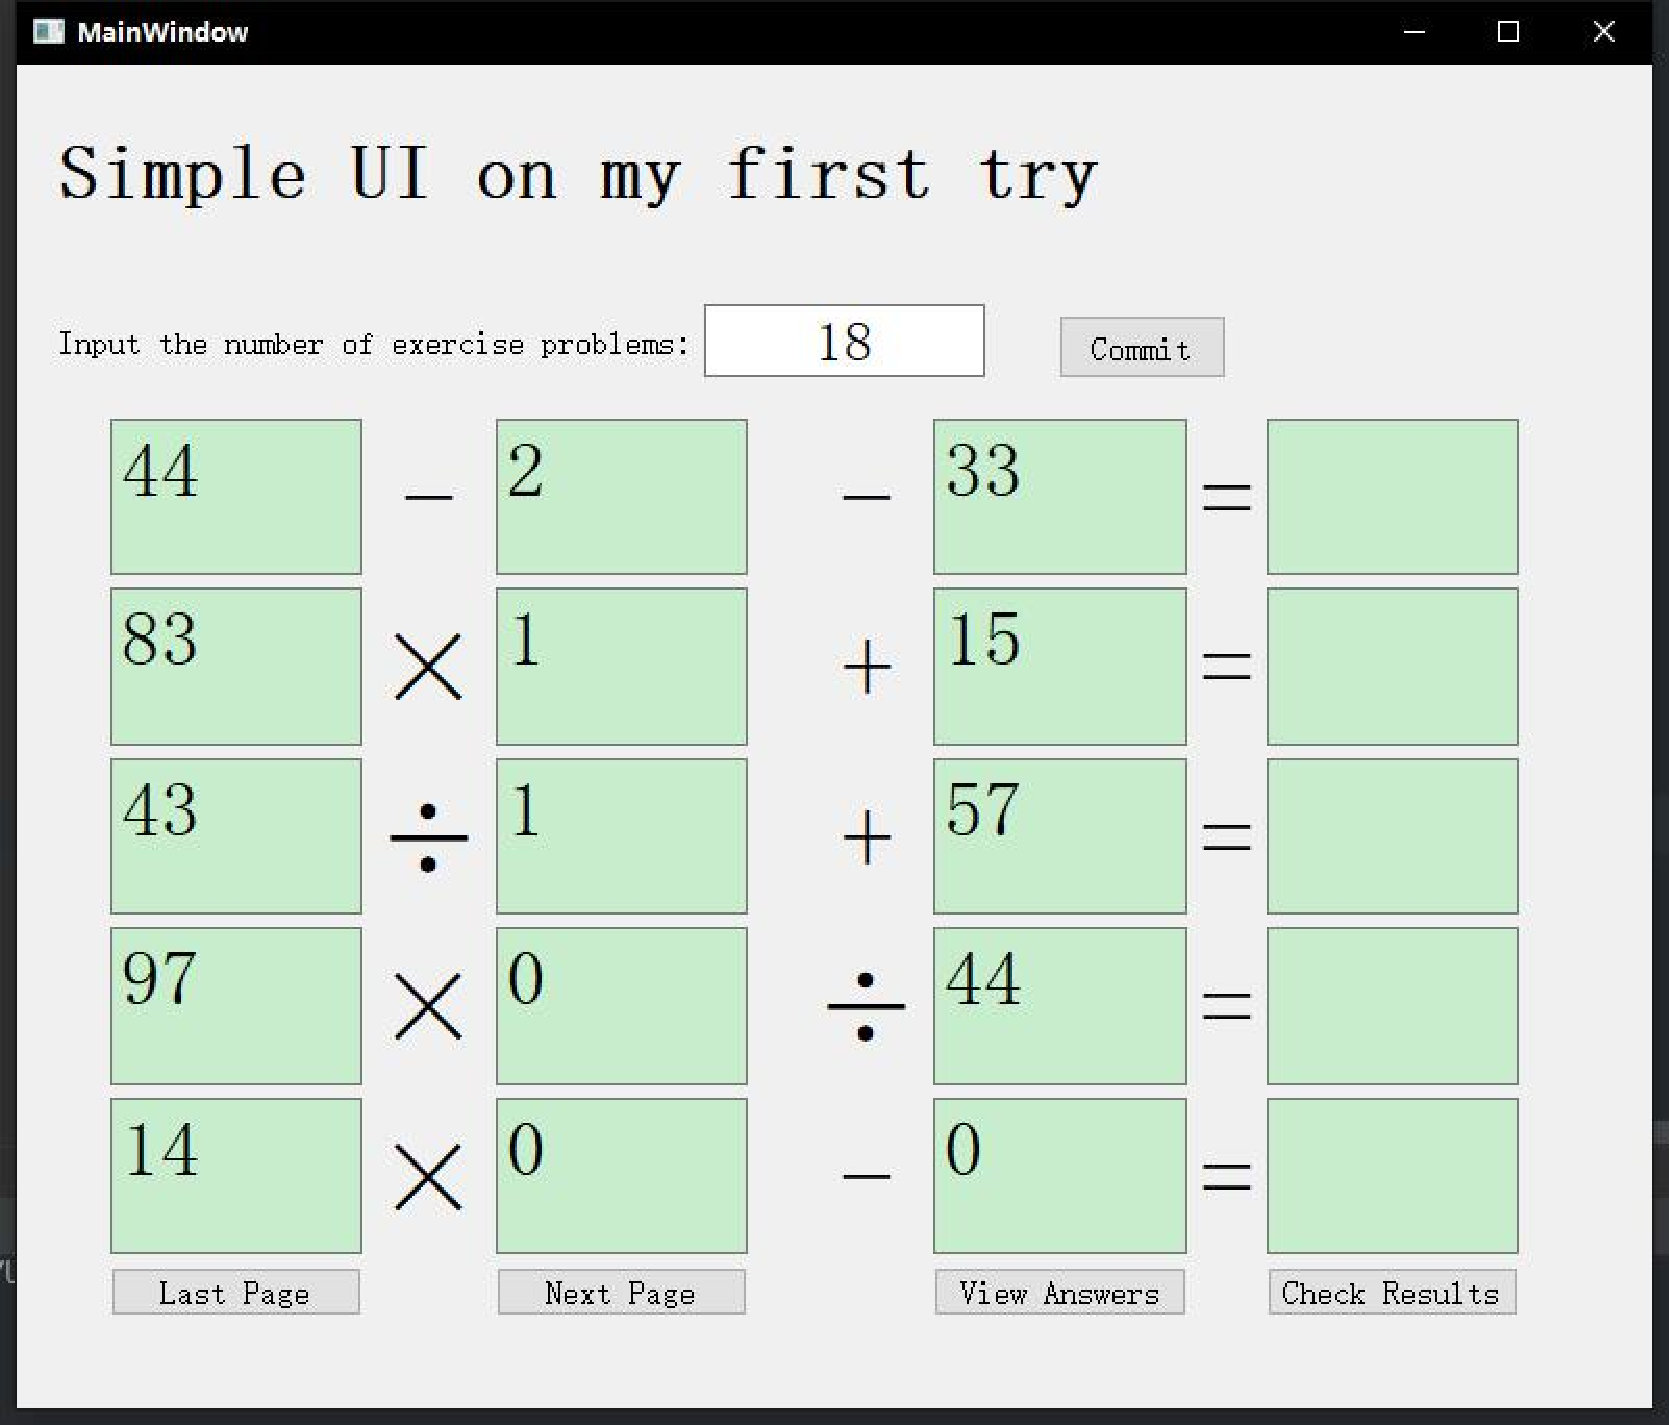
\includegraphics[width=2.5in]{./figures/next_page.pdf}
  \caption{next page}
  \label{next_page}
\end{figure}
\noindent 6.下一页,点击 last page按钮(Fig. \ref{last_page}):
\begin{figure}[H]
  \centering
  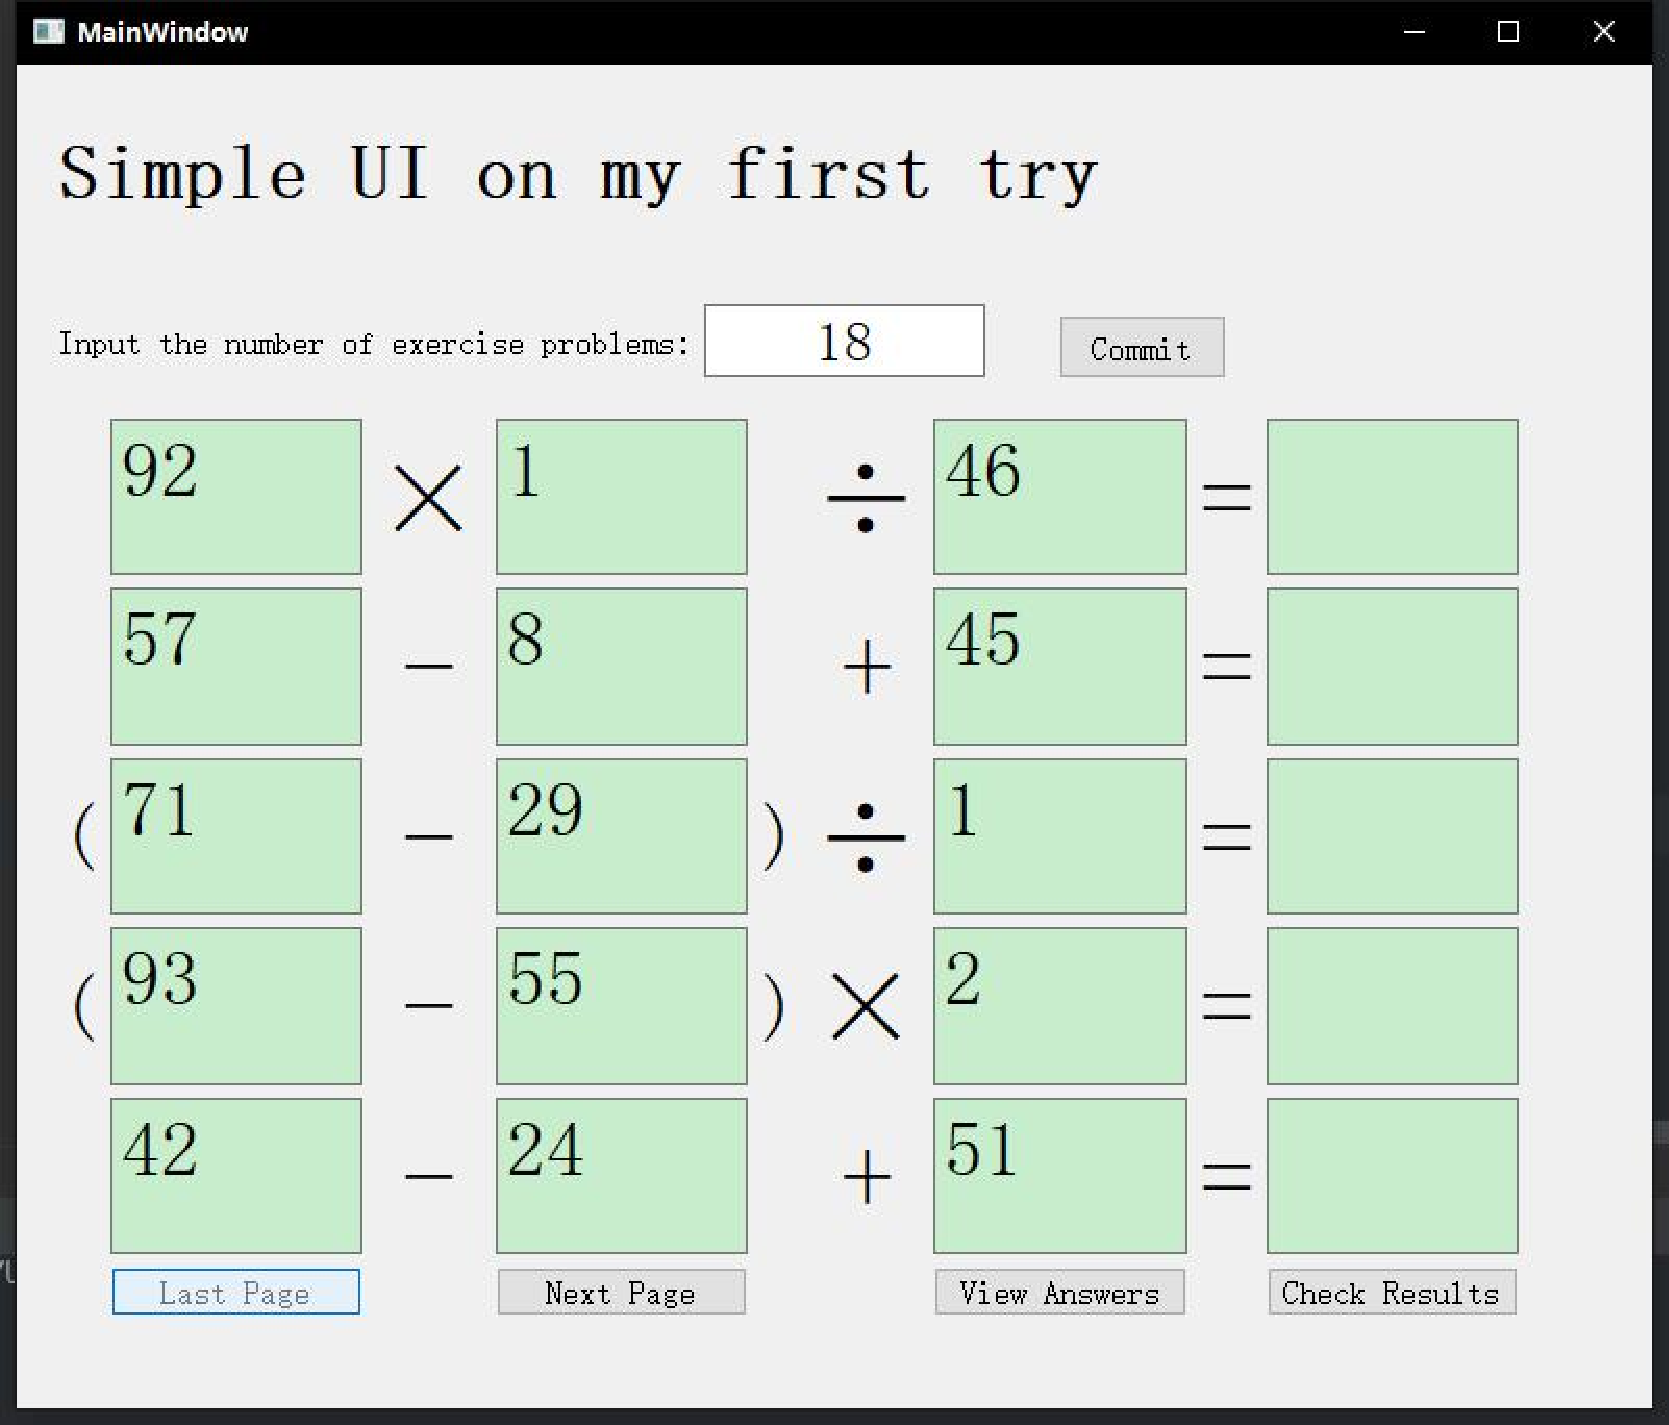
\includegraphics[width=2.5in]{./figures/last_page.pdf}
  \caption{last page}
  \label{last_page}
\end{figure}
\noindent 7.最后一页(Fig. \ref{end_page}):
\begin{figure}[H]
  \centering
  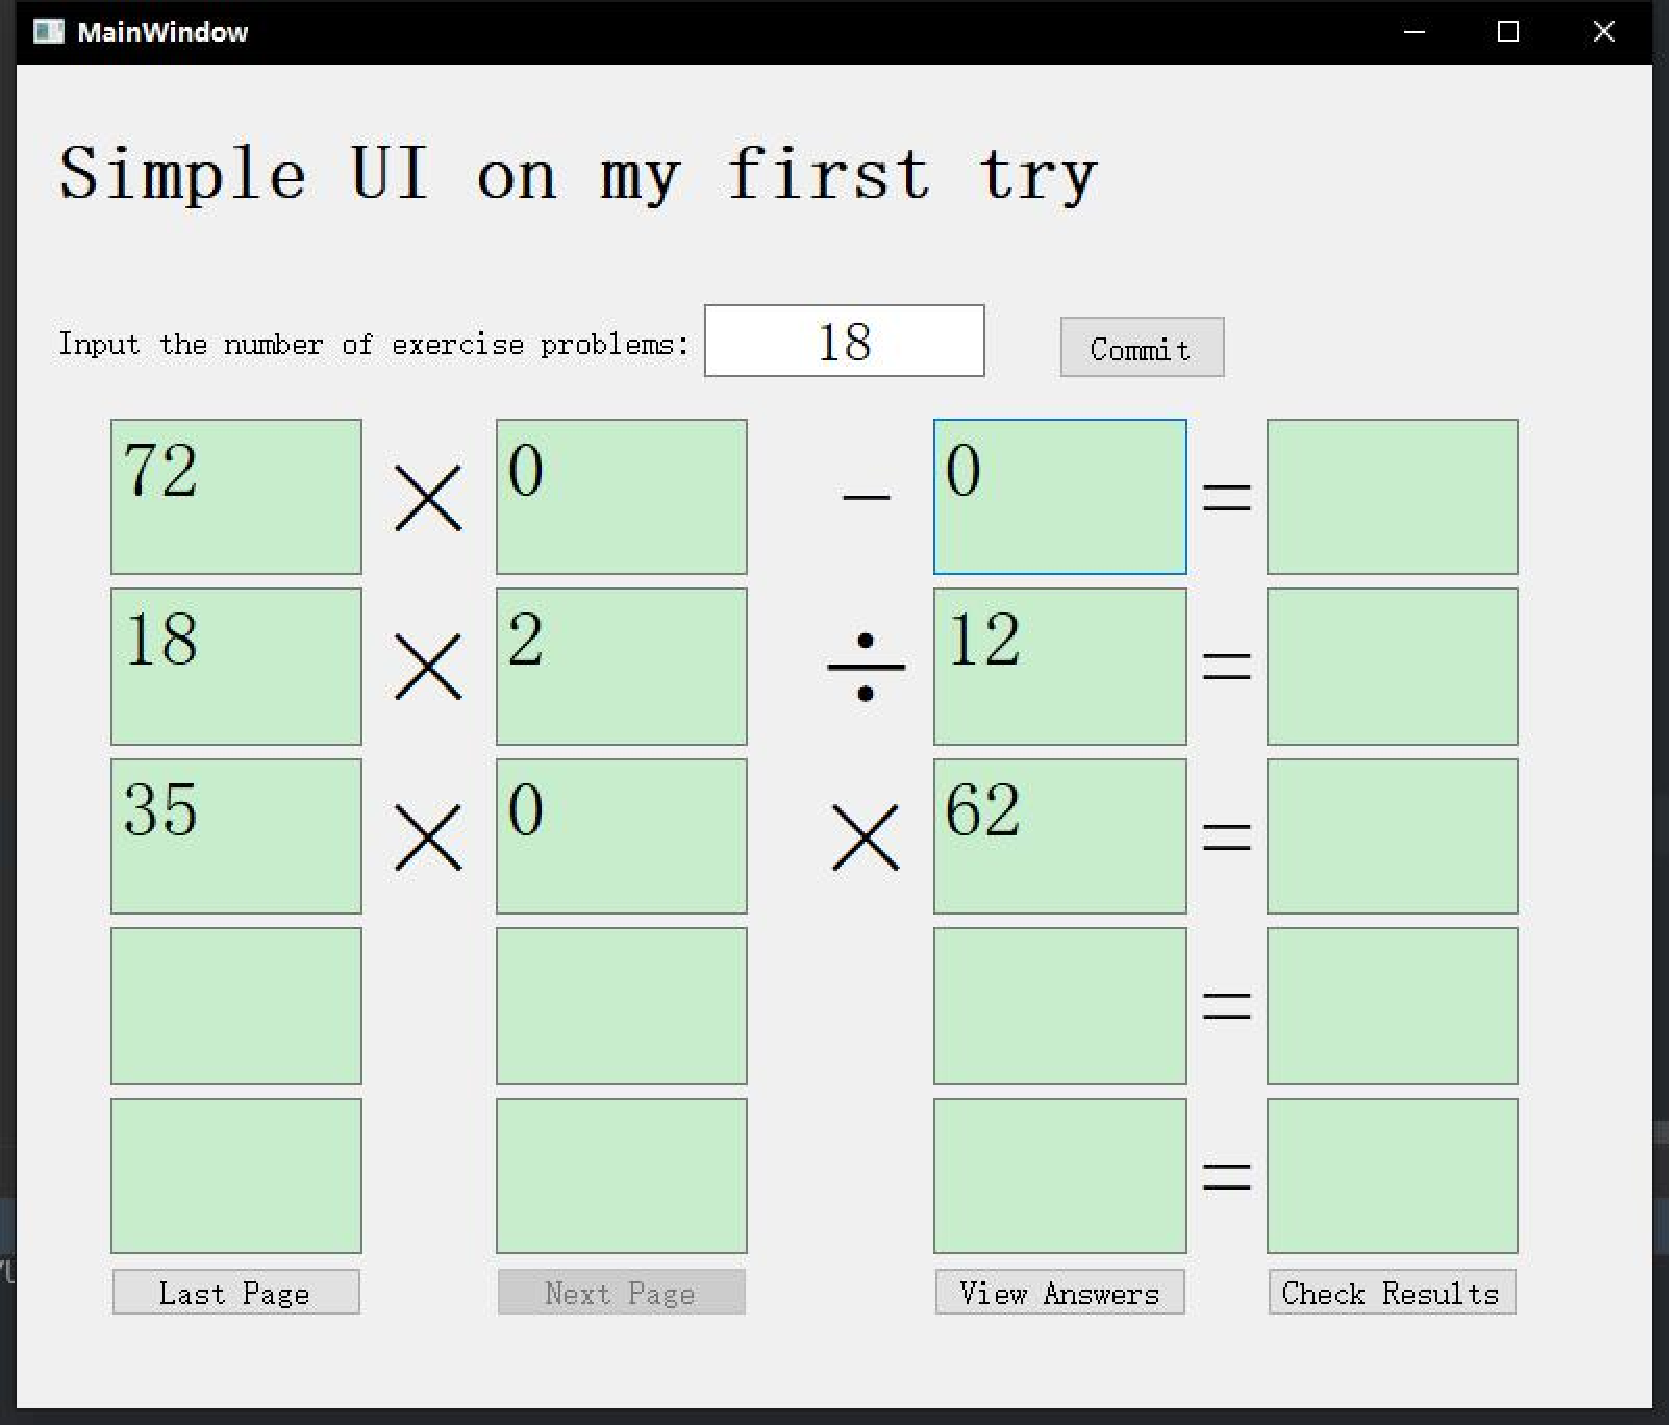
\includegraphics[width=2.5in]{./figures/end_page.pdf}
  \caption{end page}
  \label{end_page}
\end{figure}
\noindent 8.输入题目数非法(Fig. \ref{illegal_num}):
\begin{figure}[H]
  \centering
  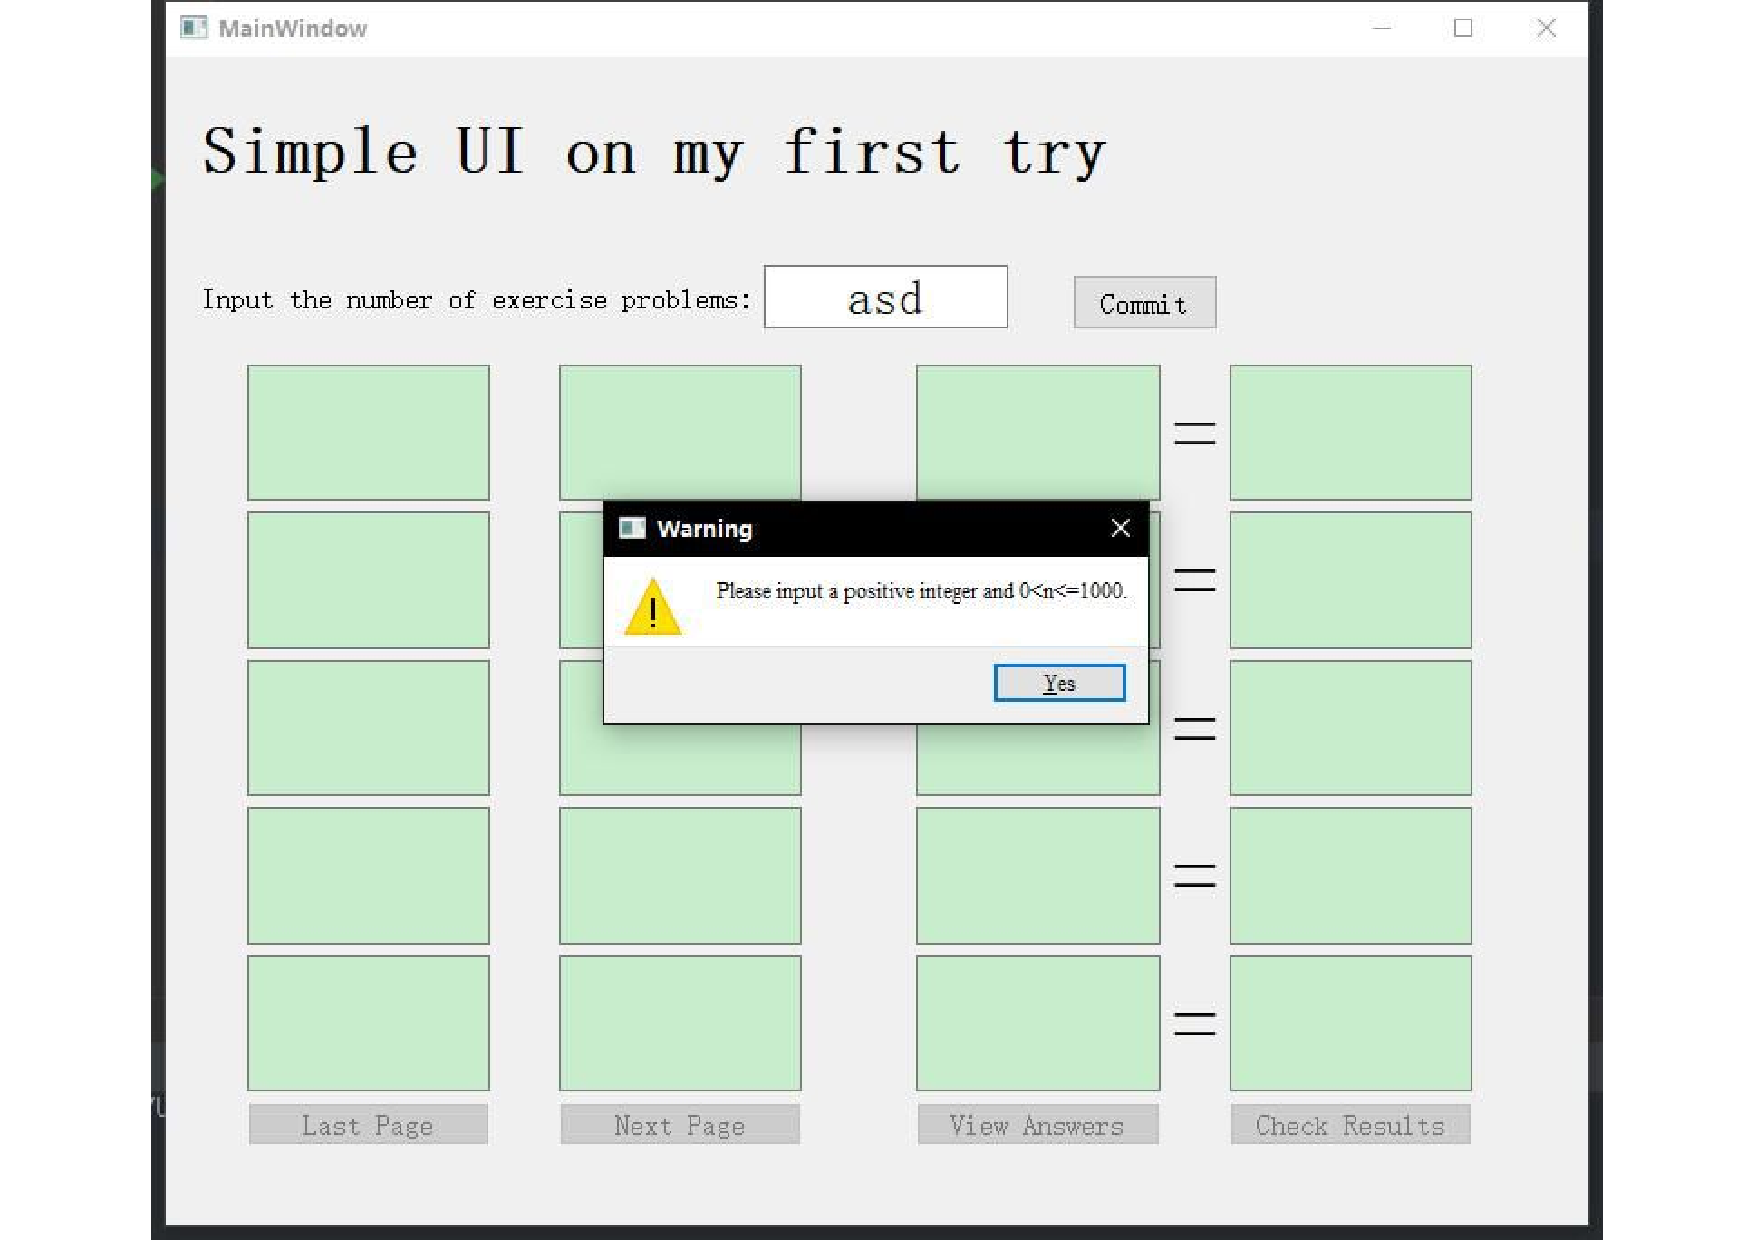
\includegraphics[width=2.5in]{./figures/illegal_num.pdf}
  \caption{illegal number}
  \label{illegal_num}
\end{figure}
\noindent 9.答案为字符串(Fig. \ref{illegal_answer}):
\begin{figure}[H]
  \centering
  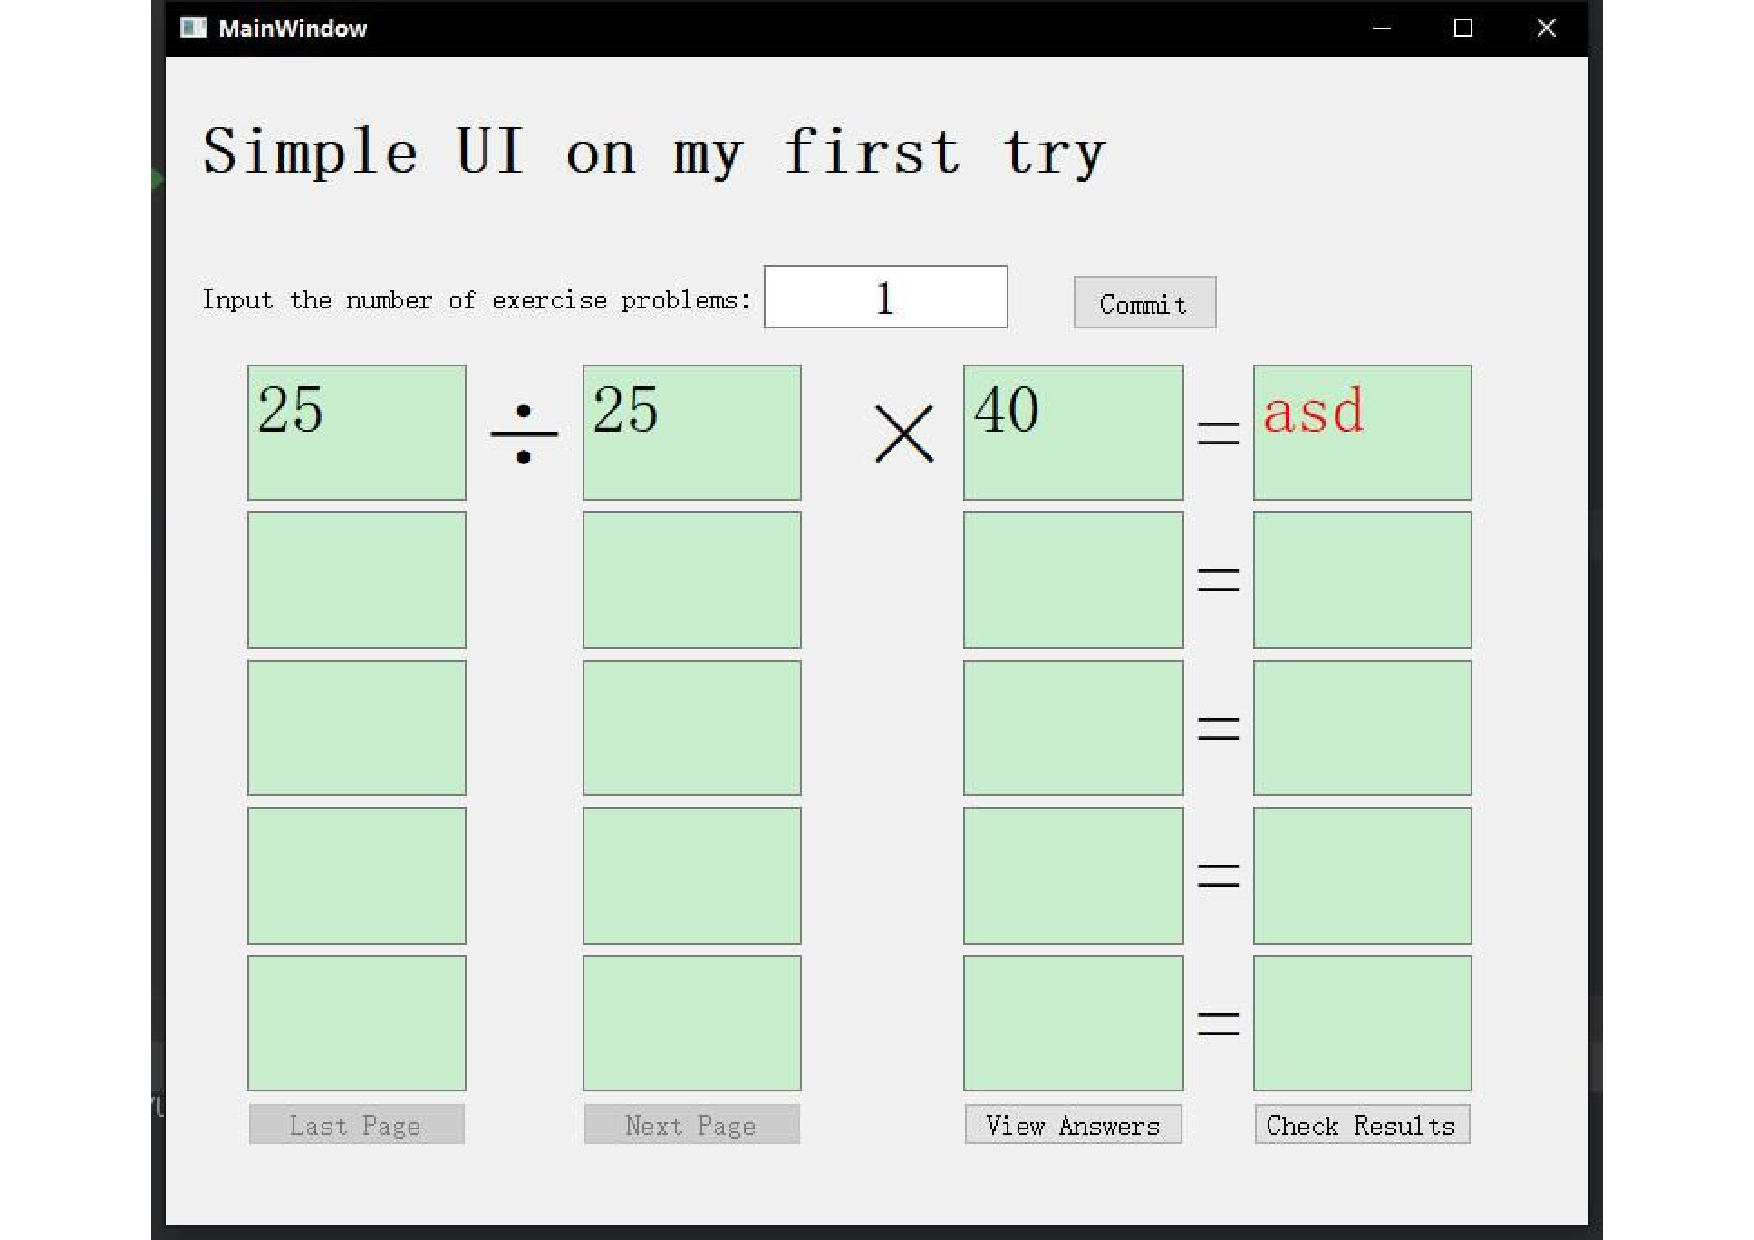
\includegraphics[width=2.5in]{./figures/illegal_answer.pdf}
  \caption{illegal answer}
  \label{illegal_answer}
\end{figure}

\end{CJK}
\end{document} 